\chapter{MOSFETs}
A transistor comes from the two words \textbf{trans}conductance res\textbf{istor}. MOSFET stands for MOS field effect transistor since we are taking the MOS CAP and adding two extra diffusion regions. Most of the EE105 reader spents time on the NMOS device since most of the concepts can be carried over into analyzing the PMOS device too. A MOSFET is a three terminal device, so we are moving on form the junction diode, a basic two terminal device

Part of the motivation for learning about MOSFETs is for building a current source and also for voltage amplification. If we are able to form a voltage controlled current source, we can build a voltage amplifier.

\section{Structure}
\begin{gline}
    \item $n^+$: heavily doped $n$-type silicon
    \item $n^-$: lightly doped $n$-type silicon
    \item $V_t$: threshold voltage
    \item $V_T$: thermal voltage
    \item $L$: channel length
\end{gline}

\begin{figure}[htb]
    \centering
    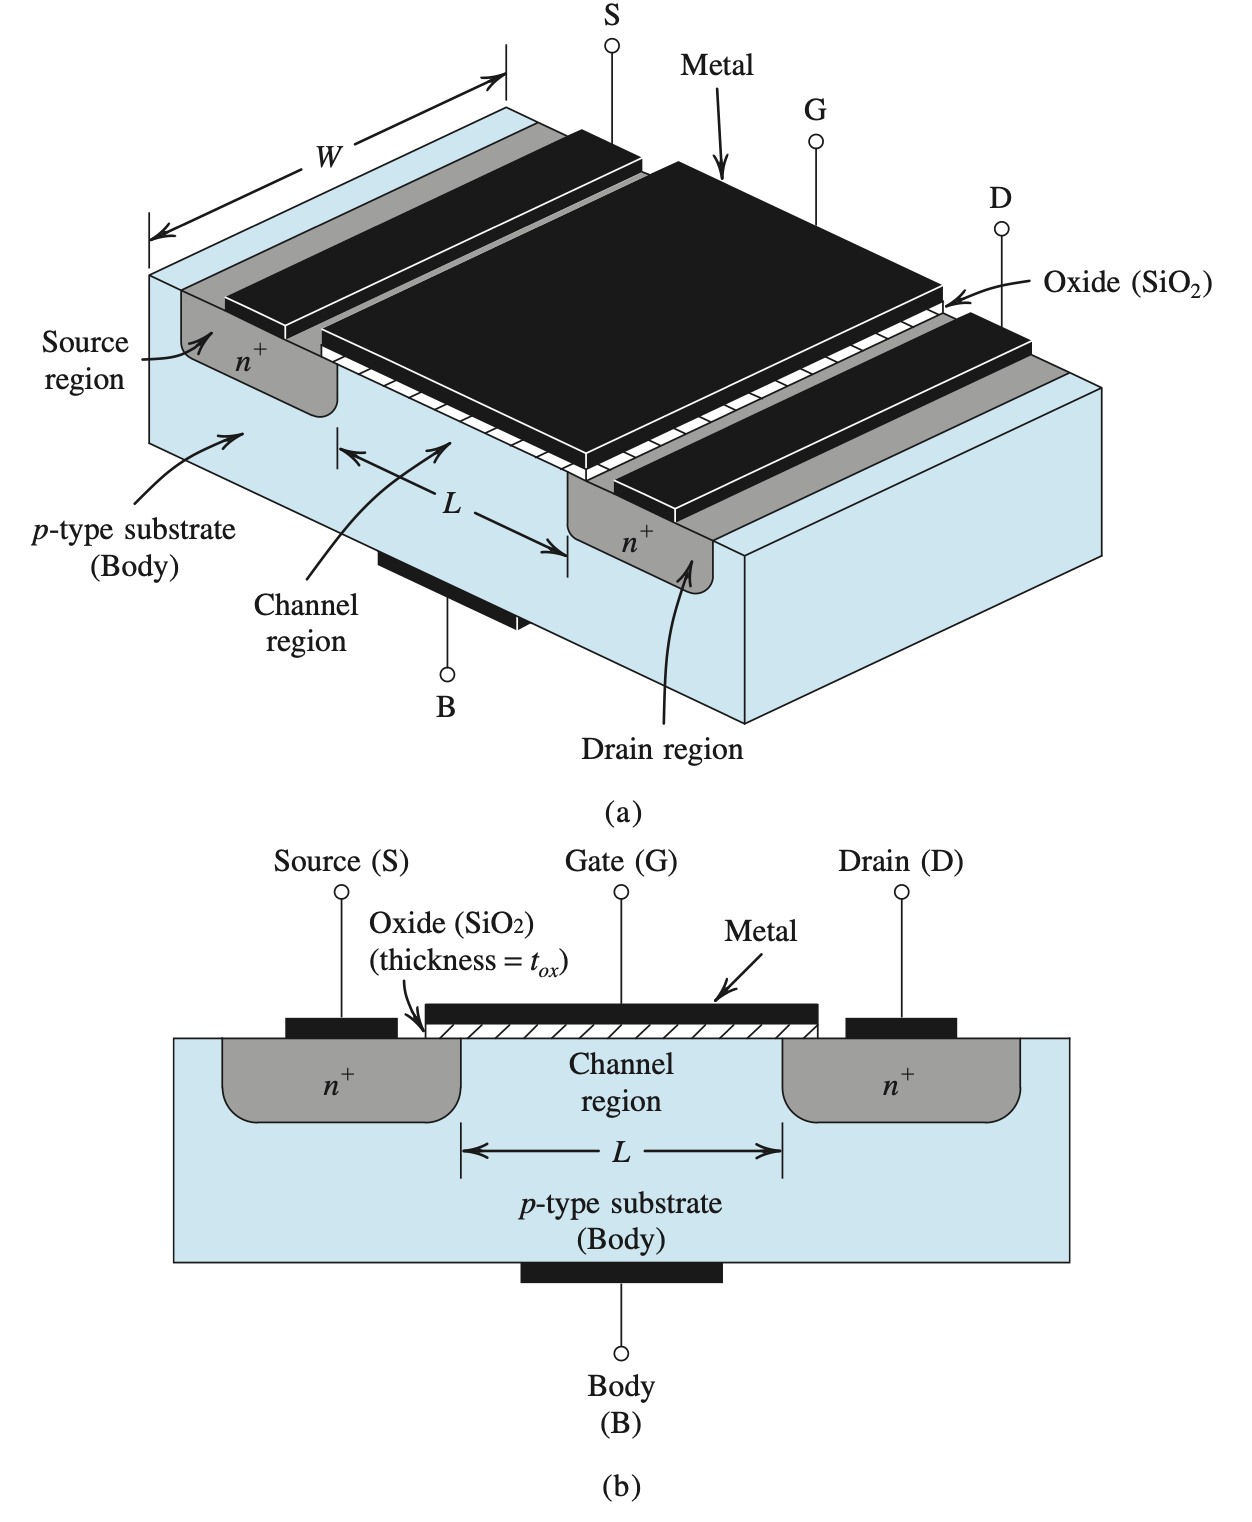
\includegraphics[scale=0.4]{figs/ch05/nmos_structure.png}
    \caption{Physical structure of the NMOS transistor and a cross section view}
    \label{fig:nmos_structure}
\end{figure}
In figure \ref{fig:nmos_structure}, we see that the NMOS transistor has the gate, source, drain, and substrate/body terminal, as indicated by the first letters of each terminal. From its physical structure, we notice that a MOSFET is a symmetrical device and that the substrate forms a PN junction with the source and drain regions.

At zero gate voltage, we see that there are two back to back diodes in series between drain and source. One from the PN junction formed between the $n^+$ drain region and the $p$ type substrate and the other from the $n^+$ source region and the $p$ type substrate. These diodes prevent current conduction from drain to source when a voltage $v_{ds}$ is applied.

\section{NMOS: Current conduction}
Suppose you ground the source and drain and $v_g > 0$. A positive gate voltage causes free holes to be repelled to the region of the substrate under the gate into the substrate. This leaves a \textbf{carrier-depletion region}. A positive gate voltage also attracts electrons from the $n^+$ source and drain regions to the channel region. Show in figure \ref{fig:nmos_conduct}
\begin{figure}[H]
    \centering
    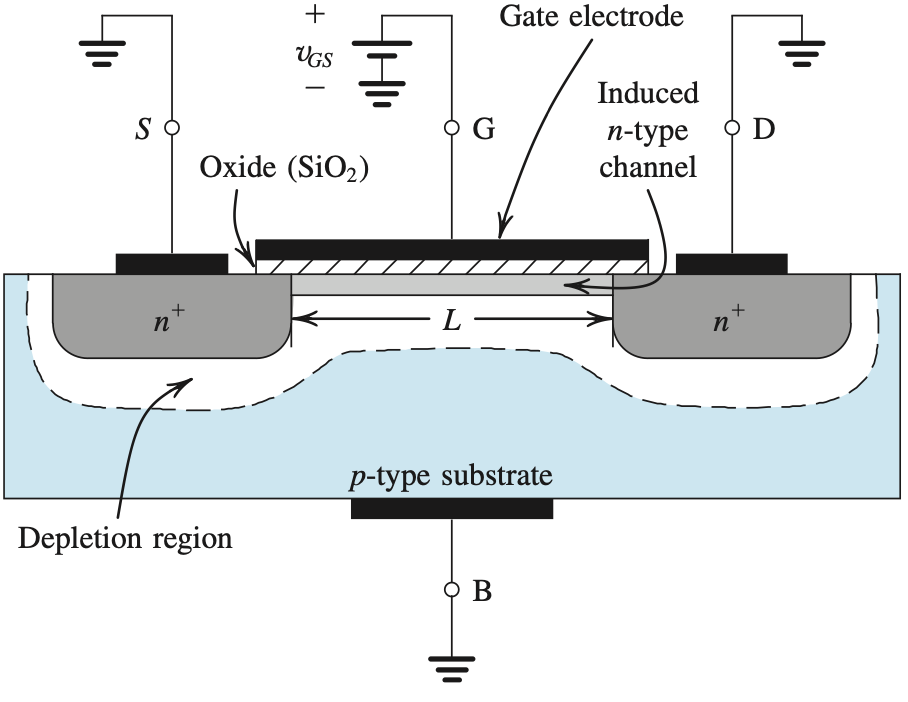
\includegraphics[scale=0.4]{figs/ch05/nmos_conduct}
    \caption{Positive voltage applied to the gate. An $n$ channel is induced at the top of the substrate beneath the gate}
    \label{fig:nmos_conduct}
\end{figure}
We see that a \textbf{channel} is formed for current flow from the drain to source. \textbf{Threshold voltage} is also defined as the value of \vgs where a sufficient number of mobile electrons accumulate in the channel region to form a conducting channel. \textbf{Overdrive voltage}, or \textbf{effective voltage} is the excess of \vgs over $V_t$. 
    \[v_{gs} - V_t \equiv v_{ov}\]
As \vov increases, so does the magnitude of the channel charge. If drawn out, this looks like the an increase in the depth/deepness of the channel.

Another thing to keep in mind here is the \textbf{oxide capacitance}.
    \[C_{ox} = \frac{\epsilon_{ox}}{t_{ox}}\]
\begin{gline}
    \item $C_{ox}$: capacitance of the parallel-plate capacitor per unit gate area, F/m\sq
    \item $\epsilon_{ox}$: permittivity of silicon dioxide; $\epsilon_{ox} = 3.9 \epsilon_0 = 3.45 \times 10^{-11}$ F/m
    \item $t_{ox}$: oxide thickness, determined by process technology
\end{gline}

\begin{Analysis}{Deriving $i_D$ for small \vds}{}
    We start by applying a small \vds and \vgs greater than its threshold voltage. $i_D$ is the current that Since $i_D$ is the charge per unit channel length, 
        \[\frac{\mid Q \mid}{\text{unit channel length}} = C_{ox} W v_{OV}\]
    We also know that channel conductance is proportional to the overdrive voltage, or \vgs $-V_t$. This means that current in the channel, $i_D$, is proportional to(\vgs $-V_t$). \vds also establishes an electric field $E$ across the length of the channel given by:
        \[\mid E \mid = \frac{v_{DS}}{L}\]
    An electric field causes channel electrons to drift towards the drain with a velocity of:
        \[\text{Electron drift velocity} = \mu_n \mid E \mid = \mu_n \frac{v_{DS}}{L}\] 
    Remembering that current is the rate of charged particles, then we find current by multiplying charge per unit channel length by the electron drift velocity.
        \[i_D = [(\mu_n C_{ox}) (\frac{W}{L}) v_{OV}] v_{DS} = [(\mu_n C_{ox}) (\frac{W}{L}) (v_{GS} - V_t)] v_{DS}\]
    Conductance of the channel is given by:
        \[g_{DS} = (\mu_n C_{ox}) (\frac{W}{L}) v_{OV} = (\mu_n C_{ox}) (\frac{W}{L}) (v_{GS} - V_t)\]
    \textbf{Process transconductance parameter} is given by:
        \[K_n' = \mu_n C_{ox}\]
\end{Analysis}

For a small \vds, the MOSFET behaves with a linear resistance $r_{DS}$ given by
    \[r_{DS} = \frac{1}{g_{DS}} = \frac{1}{(\mu_n C_{ox})(W/L)v_{OV}}\]

\begin{figure}[htb]
    \centering
    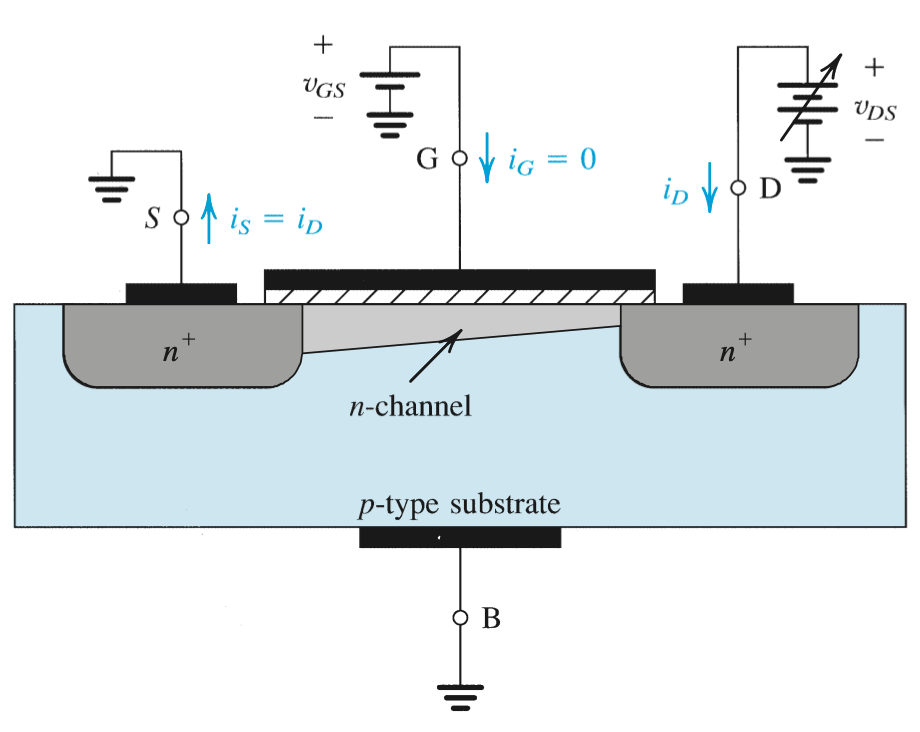
\includegraphics[scale=0.5]{figs/ch05/increase_vds.png}
    \caption{Operation of the enhancement NMOS transistor as \vds is increased}
    \label{fig:increase_vds}
\end{figure}

If we increase \vds, the depletion region will widen at the depletion region as a result of the increased \vds that makes the channel shallower near the drain. This is reflected in the formula for $i_D$. We'll see that the channel looks more like a tapered shape, where it's deepest at the source end (proportional to \vov) and shallowest at the drain end (proportional to \vov - \vds). Shown in figure \ref{fig:increase_vds}.
\[i_D = \mu_n C_{ox} (\frac{W}{L}) (V_{OV} - \frac{1}{2}v_{DS})v_{DS}\]

\begin{figure}[htb]
    \centering
    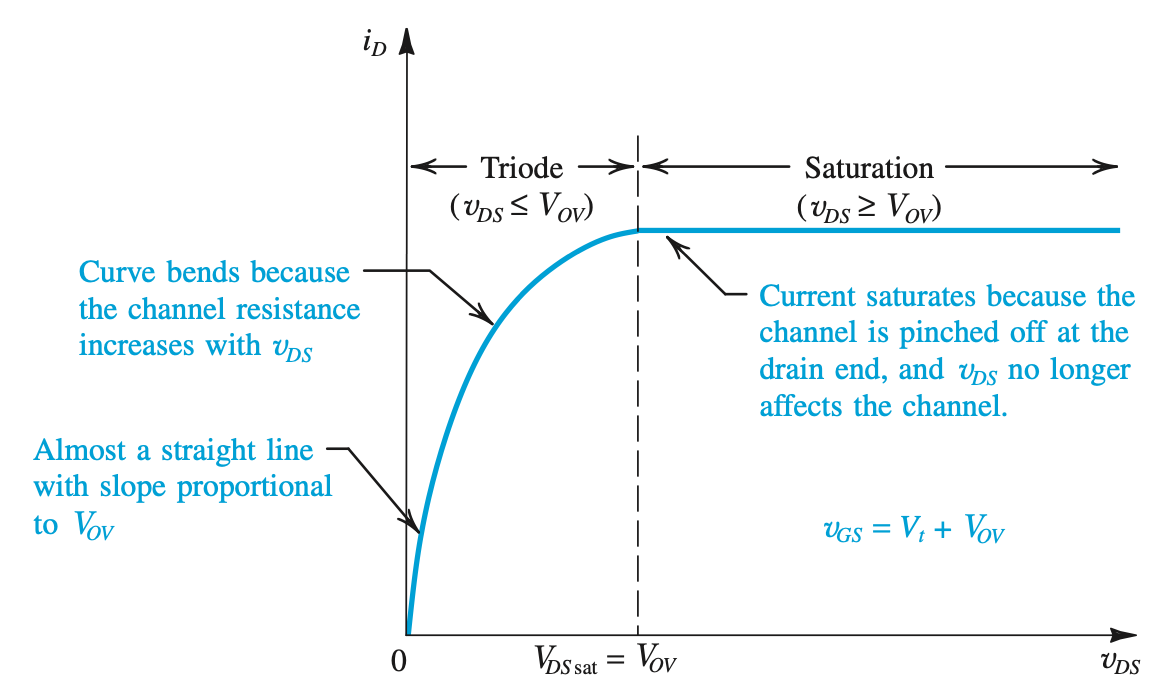
\includegraphics[scale=0.5]{figs/ch05/pinch_off.png}
    \caption{Operation of the enhancement NMOS transistor in different regions}
    \label{fig:pinch}
\end{figure}

Figure \ref{fig:pinch} shows the drain current for different regions. Increasing \vds beyond \vov has no affect on the channel shape and charge. This is when the transistor enters saturation and the channel region resembles a right triangle with the deepest part being close to the source.

\section{PMOS: Structure and Current conduction}
\begin{figure}[htb]
    \centering
    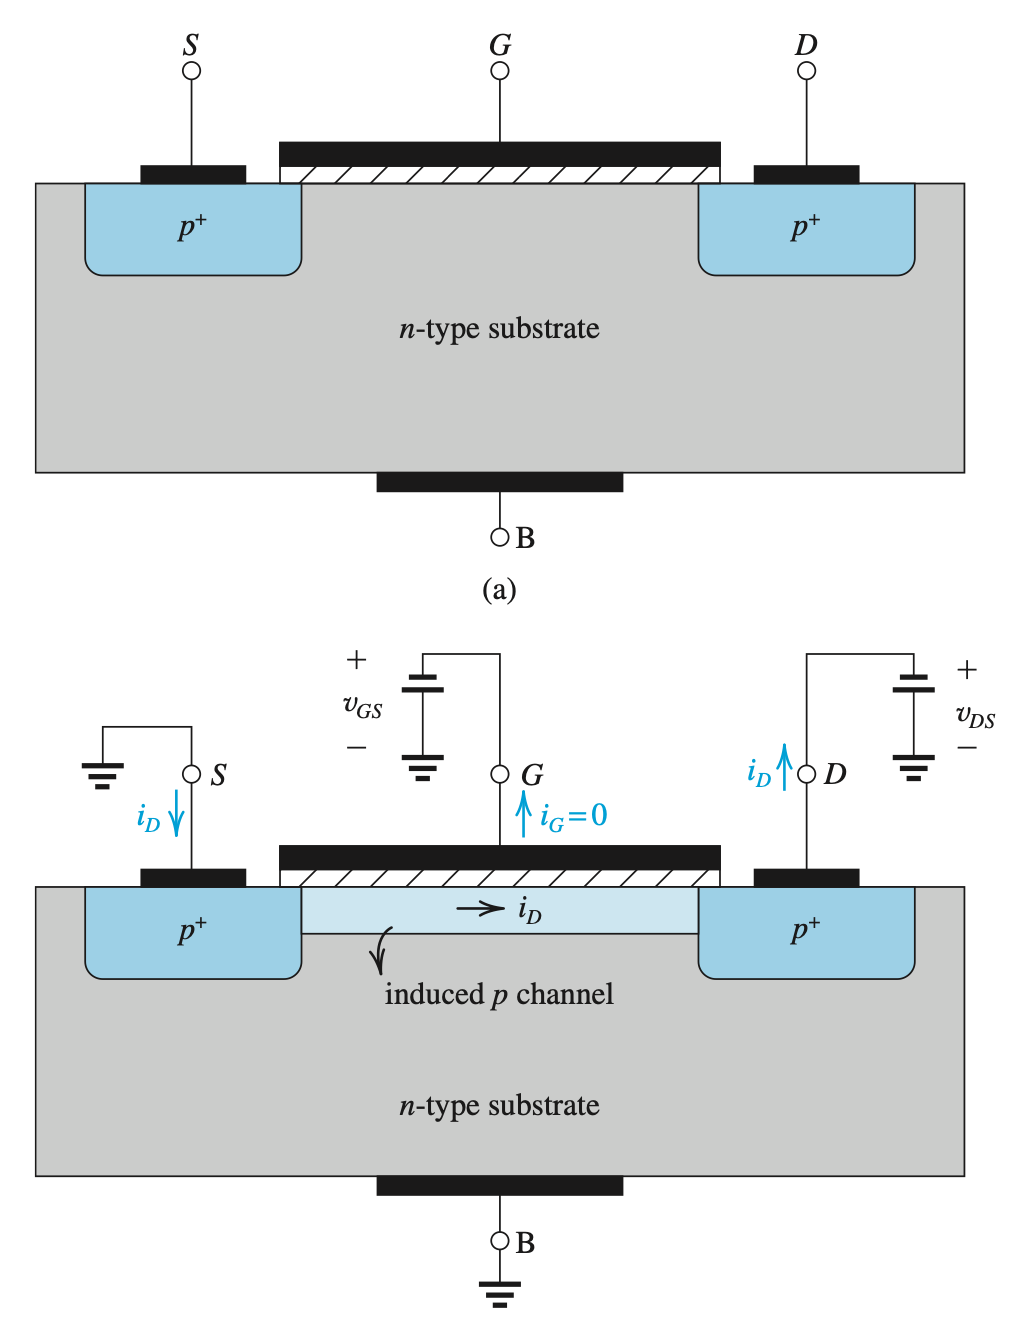
\includegraphics[scale=0.5]{figs/ch05/pmos_structure.png}
    \caption{Physical structure of the PMOS structure and side view}
    \label{fig:pmos_structure}
\end{figure}
To conduct current here, we need to apply a negative voltage between the gate and the source. This is because the current here is carried by holes (current goes in the same direction as the holes, contrastingly from when current is carried by electrons) and flows from the source to the drain. If we had to compare the NMOS cross section with the PMOS cross section, then we would notice that the substrate type for a PMOS transistor is an $n$-type substrate with $p^+$-type wells for the source and drain, while this is switched for a NMOS transistor ($p$-type substrate with $n^+$-type wells for source and drain). We'll also notice that the direction of current is flowing from opposite wells.
\begin{gline}
    \item $k'_p = \mu_p C_{ox}$: process transconductance parameter for PMOS
    \item $mu_p$: mobility of the holes in the induced 
    \item $k_p = k'_p(W/L)$: transistor transconductance parameter
\end{gline}

Typically, NMOS transistors have greater gain and speed of operations than PMOS devices. Electron mobility $\mu_n$ is higher by factor of 2 to 4 than the hole mobility $\mu_p$. The following attached PDF was something found online but sums up everything pretty nicely in a funny style.

\newpage %commenting this out for now so that its not so intensive to create test pdfs
% 
\includepdf[scale=0.9, clip, trim=10mm 10mm 10mm 10mm, pages={1-10}]{chapters/Applying_drain_voltage_nmos.pdf}


\section{Large and Small Signal Equivalent Models}
Large signal equivalent model of an $n$-channel MOSFET operating in the saturation region
\begin{figure}[H]
    \centering
    % \begin{circuitikz}[american voltages]
    %     \draw
    %       (0,0) to [short, o-] (6,0)
    %       to [V, l_=$\mathrm{j}{\omega}_m \underline{\psi}^s_R$] (6,2) 
    %       to [R, l_=$R_R$] (6,4) 
    %       to [short, i_=$\underline{i}^s_R$] (5,4) 
    %       (0,0) to [open, v^>=$\underline{u}^s_s$] (0,4) 
    %       to [short, *- ,i=$\underline{i}^s_s$] (1,4) 
    %       to [R, l=$R_s$] (3,4)
    %       to [L, l=$L_{\sigma}$] (5,4) 
    %       to [short, i_=$\underline{i}^s_M$] (5,3) 
    %       to [L, l_=$L_M$] (5,0); 
    % \end{circuitikz}
    \begin{circuitikz}[american voltages]
        \draw 
        (0,0) coordinate(a) 
            to [short, o-o] ++(10,0) 
        coordinate(b) 
            to (a) 
            to [open, -o] ++(0,2) coordinate(c)
            to [short,-o, i=$i_G$] ++(1,0)
            to [open, v=$v_{GS}$] ++(0,-2)
            to (b)
            to [open, v<=$v_{DS}$] ++(0,2) coordinate(d)
            to [short, i=$i_D$] ++(-1,0)
            to [short] ++(-6,0)
            to [cI, -*, l=$\frac{1}{2} k'_n \frac{W}{L}(v_{GS} - V_{tn})^2$] ++(0,-2)
            to ++(-1,0)
            to [short, *-o, l=S] ++(0,-0.5)
            to [open, -*] ++(6,0.5)
            to [R, -*, l_=$r_o$] ++(0,2)
            ;
    \end{circuitikz}
    \caption{Large signal model operating in saturation drawn with outputresistance $r_o$}
\end{figure}

\section{A More Complete Model}

\begin{figure}[H]
    \centering
    \begin{circuitikz}[scale=0.6, american voltages]
        \ctikzset{bipoles/resistor/height=0.15}
        \ctikzset{bipoles/resistor/width=0.4}
        \ctikzset{bipoles/capacitor/height=0.35}
        \ctikzset{bipoles/capacitor/width=0.1}
        \coordinate (G) at (0,0);
        \coordinate (D) at (14,0);
        \coordinate (S) at (0,-3);
        \coordinate (B) at (0,-6);
        \coordinate (curr1) at (4,0);
        \coordinate (curr2) at (7.75,0);
        \coordinate (res) at (11,0);
        \coordinate (Cdb) at (13,0);
        \draw 
        (G) 
            to [short, o-*] ++(1,0) node[label=left:G] at (G){}
            to [C, -*, l=$C_{gd}$] (curr1)
            to [short, -*] (curr2) 
            to [short, -*] (res)
            to [short, -*] (Cdb)
            to [short, -o] (D) node[label=right:D] {}
            to [open, i=$i_{ds}$] ++(-3,0)
        (G) 
            to [open] ++(1,0)
            to [C, -*, l=$C_{gs}$, v=$v_{gs}$] ++(0,-3)
            to [C, -*, l=$C_{sb}$, v<=$v_{bs}$] ++(0,-3)
        (S)
            to [short, o-*] ++(1,0) node[label=left:S] at (S){}
        (B)
            to [short, o-*] ++(1,0) node[label=left:B] at (B){}
            to ++(12,0)
        (curr1)
            to [cI, -*, l=$g_m v_{gs}$] ++(0,-3)
        (curr2)
            to [cI, -*, l=$g_{mb} v_{bs}$] ++(0,-3)
        (res)
            to [R, l=$r_o$] ++ (0,-3)
            to (S)
        (Cdb)
            to [C, l=$C_{db}$] ++(0,-3)
            to ++(0,-3)
            to (B)
        ;
    \end{circuitikz}
    \caption{A more complete NMOS model that is complete with capacitances.}
\end{figure}

With this model, we can rewrite \ids as the following:
    \[i_{DS} = g_m v_{gs} + g_{mb} v_{bs} + \frac{1}{r_o} v_{ds}\]
We see that the more complete model for the PMOS transistor is also really similar with some minor differences

\begin{figure}[H]
    \centering
    \begin{circuitikz}[scale=0.6, american voltages]
        \ctikzset{bipoles/resistor/height=0.15}
        \ctikzset{bipoles/resistor/width=0.4}
        \ctikzset{bipoles/capacitor/height=0.35}
        \ctikzset{bipoles/capacitor/width=0.1}
        \coordinate (S) at (0,0);
        \coordinate (D) at (15,-3);
        \coordinate (G) at (0,-3);
        \coordinate (B) at (0,-6);
        \coordinate (curr1) at (4,0);
        \coordinate (curr2) at (7.75,0);
        \coordinate (res) at (11,0);
        \coordinate (Cdb) at (13,-3);
        \draw 
        (G) 
            to [short, o-*] ++(1,0) node[label=left:G] at (G){}
            to [C, -*, l=$C_{gd}$] ++(3,0)
            to (D)
            to [short, -o] (D) node[label=right:D] {}
            to [open, i<=$i_{ds}$] ++(-3,0)
        (G) 
            to [open] ++(1,0)
            to [C, -*, l=$C_{gs}$, v<=$v_{sg}$] ++(0,3)
            % to [C, -*, l=$C_{sb}$, v<=$v_{bs}$] ++(0,3)
        (S)
            to [short, o-*] ++(1,0) node[label=left:S] at (S){}
            to (res)
        (B)
            to [short, o-*] ++(1,0) node[label=left:B] at (B){}
            to ++(12,0)
        (curr1)
            to [cI, *-*, l=$g_m v_{sg}$] ++(0,-3)
        (curr2)
            to [cI, *-*, l=$g_{mb} v_{sb}$] ++(0,-3)
        (res)
            to [R, -*, l=$r_o$] ++ (0,-3)
        (Cdb)
            to [C, *-, l=$C_{db}$] ++(0,-3)
            to (B)
            to ++(1,0)
            to [C] ++(0,3)
        ;
    \end{circuitikz}
    \caption{A more complete NMOS model that is complete with capacitances.}
\end{figure}

How does this more complete model affect the amplification effect?

Future chapters will talk about the BJT (bipolar junction transistor). 
\begin{pline}
    \item MOSFETs can be made smaller than BJTs
    \item MOSFET manufacturing process is relatively simpler and requires comparatively little powers
    \item MOSFETs generate less heat
    \item BJT better for current amplification circuits
    \item BJT low on-state voltage drop and low conduction loss
    \item BJT preferred in high power applications due to higher power handling; MOSFET preferred for low power applications
\end{pline}

\begin{todo}
    \item reorganize these items into a gline into the appropriate section
    \item $C_{gs}$: gate-source capacitance in saturation
    \item $C_{ov}$: MOSFET parasitic overlap capacitance
    \item $C_{gd}$: gate-drain capacitance in saturation
    \item $C_{sb}$: source body capacitance
    \item $C_{db}$: drain body capacitance
    \item also make tex model for mosfet with the body capacitances and a complete model (lec4/4/24)
\end{todo}
\section{Practice Problems}
\begin{enumerate}
    \item Find the region of operation for the following transistors. You may use $V_{tn} = 0.9$V and $\mid V_{tp} = 1$V. The operation condition of NMOS is also shown. PMOS is conducted by holes which is opposite to NMOS so the voltage polarity is different.
    \begin{figure}[H]
        \centering
        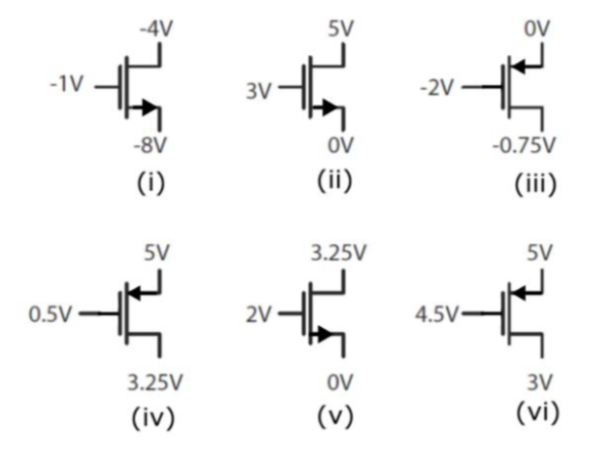
\includegraphics[scale=0.8]{figs/ch05/pp_transistor1.png}
    \end{figure}
    \begin{center}
        \begin{tabular}{|c|c|c|}
            \hline
            Region of operation & Condsitions & \ids \\
            \hline
            Cut-off & \vgs < $V_T$ & \ids $\sim$ 0A \\
            \hline
            Linear/Triode & $V_{GS}$ > $V_T$, $V_{DS} < V_{GS} - V_T$ & \ids = {\large $\frac{W}{L} \mu_n C_{ox} (V_{GS} - V_T - \frac{V_{DS}}{2}) V_{DS}$} \\ [10pt]
            \hline
            Saturation: & $V_{GS}$ > $V_T$, $V_{DS} > V_{GS} - V_T$ & {\large \ids = $\frac{W}{L} \frac{\mu_n C_{ox}}{2} (V_{GS} - V_T)^2 (1+ \lambda V_{DS})$} \\
            \hline
        \end{tabular}
    \end{center}
    \textcolor{blue}{
    \begin{enumerate}
        \item We identify this transistor as a NMOS transistor due to the direction of the arrow. In a NMOS transistor, current flows from drain to source due to electrons being the charge carriers in the NMOS transistor. \vgs = $v_G - v_S$ = 7V and \vds = $v_D - v_S = -4 -(-8) - 4$V. This transistor is in the linear/triode region. 
        \item \vgs = 3V and \vds = 5V. This transistor is in the saturation region.
        \item This is a PMOS transistor. In a PMOS transistor, current flows from source to drain. $|v_{GS}|= 2$V and $|v_{DS}|= 0.75$V. This is in the linear/triode region.
        \item $|v_{GS}| = 4.5$V and $|v_{DS}| = |3.25 - 5| = 1.75$V. This is in the linear/triode region.
        \item $v_{GS} = 2$V and $v_{DS} = 3.25-0 = 3.25$V. This is in the saturation region.
        \item $|v_{GS}| = |4.5-5| = 0.5$V. This is in the cutoff region.
    \end{enumerate}
    }

    \item An ideal $N$-channel MOSFET has the following parameters: $W = 100$ \mun, $L = 1$ \mun, $t_{ox} = 15$ nm, the oxide relative permittivity is 4, the silicon relative permittivity is 12, $N_A = 10^{15}$\conc, $n_i = 10^{10}$\conc, $V_{FB} = -0.2$ V, $\mu_n = 300$\mobility at 300K. $\lambda = 0$.
    \begin{enumerate}
        \item Find the threshold voltage.
        \begin{Ans}
            Threshold voltage is given by the following formula:
            \begin{align*}
                \phi_B &= \frac{kT}{q} \ln\frac{N_A}{n_i} = 0.026 V \ln(\frac{10^{15} \mathrm{ cm}^{-3}}{10^{10} \mathrm{ cm}^{-3}}) = 0.2993 \dots V \\
                C_{ox} &= \frac{\epsilon_{ox}}{t_{ox}} = \frac{4(8.854 \times 10^{-14} \mathrm{F/cm})}{15 \mathrm{nm}} = 3.54 \times 10^{-7} \mathrm{F/cm}^2 \\
                V_t &= V_{FB} + 2\phi_B + \frac{\sqrt{2q\epsilon_s N_A 2 \phi_B}}{C_{ox}} \\
                &= -0.2 + 2(0.299) + \frac{2(12)(8.854 \times 10^{14} \mathrm{F/cm})(1.602 \times 10^{-19} C)(10^{15} \mathrm{cm}^{-3})(2)(0.2993 V)}{3.54 \times 10^{-7} \mathrm{F/cm}^2} \\
                &= 0.44 \mathrm{V}
            \end{align*}
        \end{Ans}

        \item What is the minumum \vds value for the MOSFET to be at saturation region at \vgs = 2V. 
        \begin{Ans}
            For the MOSFET to remain in saturation, \vds = \vgs - $V_tn$, so 
            \[V_{DS} - V_{DS} - V_{tn} = 2 - 0.44 = 1.56 \mathrm{V}\]
        \end{Ans}

        \item Find the channel resistance at \vgs = 2V and \vds = 0.01 V.
        \begin{Ans}
            Channel resistance is given by calculating what \ids is given that we know \vds is. 
            \begin{align*}
                R_{ch} &= \frac{V_{DS}}{I_{DS}} = \frac{0.01 V}{\frac{W}{L} \mu_n C_{ox} (V_{GS} - V_T) V_{DS}} \\
                &= \frac{1}{300 \times 100 \times 3.54 \times 10^{-7} \times 1.56} \\
                &= 60.36 \Omega
            \end{align*}
        \end{Ans}

        \item Find $I_D$ at \vgs = 2V and \vds = 1V.
        \begin{Ans}
            At these values, the transistor is in the linear/triode region, so 
            \begin{align*}
                I_D &= \frac{\mu_n W}{L} C_{ox} ((v_{GS} - V_{tn}) v_{DS} - \frac{v_{DS}^2}{2}) \\ 
                &= 300 \times 100 \times 3.54 \times 10^{-7}(2 - 0.44) (1 - \frac{1^2}{2}) \\
                &= 0.011 A
            \end{align*}
        \end{Ans}        

        \item Find $I_D$ at \vgs = 2V and \vds = 2V.
        \begin{Ans}
            At these values, the transistor is in the saturation region.
            \begin{align*}
                I_D &= \frac{\mu_n W}{2 L} C_{ox} (v_{gs} - v_t)^2 \\
                &= \frac{300}{2} \times 100 \times 3.54 \times 10^{-7} \times (2-0.44)^2 \\
                &= 0.013 A
            \end{align*}
        \end{Ans}
    \end{enumerate}

    \item A circuit designer intending to operate a MOSFET in saturation is considering the effect of changing the device dimensions and operating voltages on the drain current $I_D$. Specifically, by what factor does $I_D$ change in each of the following cases?
    \begin{enumerate}
        \item The channel length is doubled.
        \begin{Ans}
            The problem says that the MOSFET is in saturation. $I_D$ in saturation is 
                \[I_D = \frac{1}{2} \mu_n C_{ox} (\frac{W}{L}) (v_{GS} - V_{tn})^2\]
            From the above equation, we see that $I_D$ is inversely proportional to channel length. So, if channel length is doubled then $I_D$ will be halved.
        \end{Ans}

        \item The channel width is doubled.
        \begin{Ans}
            $I_D$ will be doubled (refer to equation for $I_D$ in saturation above).
        \end{Ans}

        \item The overdrive voltage is doubled.
        \begin{Ans}
            Overdrive voltage is equal to \vgs - $V_t$, so $I_D$ will quadruple if the overdrive voltage is doubled.
        \end{Ans}

        \item The drain to source voltage is doubled.
        \begin{Ans}
            If we doubled \vds, there will be no effect on the drain current since \vds already reaches overdrive voltage drain current saturates and remains constant.
        \end{Ans}

        \item Changes (a), (b), (c), and (d) are made simultaneously.
        \begin{Ans}
            Simultaneously doing change (a) and change (b) results in the current remaining constant. Double the overdrive voltage results in drain current quadrupling while (d) will not change drain current so the drainc current will stay 
        \end{Ans}

        \item Which of these changes might cause the MOSFET to leave the saturation region?
        \begin{Ans}
            Decreasing \vds may cause this since this may change the channel underneath.
        \end{Ans}
    \end{enumerate}

    \item An $N$-channel MOSFET with the following parameters: $W = 10$\mun, $L = 1$\mun, $V_t  =0.5$V, $\mu_n = 400$ \mobility, \cox $=4\times10^{-7}$ F/cm\sq, $\lambda = 0.01 \mathrm{V}^{-1}$.
    
    \begin{figure}[H]
    \centering
    \begin{circuitikz}[american voltages]
        \ctikzset{tripoles/mos style/arrows}
        \coordinate (start) at (0,0);
        \draw 
        (start) node[nmos](nmos){} 
        (nmos.G) 
            to ++(-1,0) 
            to [sV, l_=$v_s$] ++(0,-1.5)
            to [V, l_=$V_{GS}$] ++(0,-1) node[ground]{}
        (nmos.S) 
            to ++(0,0) node[ground]{}
        (nmos.D) 
            to [short, *-o, l=$v_o$] ++(1,0)
        (nmos.D)
            to [R, *-*, l=$R_D$] ++(0,2)
            to ++(2,0)
            to [V, *-, v=$V_{DD}$] ++(0,-1.5) node[ground]{} 
        ;
    \end{circuitikz}
    \caption{Circuit for this problem}
\end{figure}

    \begin{enumerate}
        % STATIONARY WRAPFIGURE FORCED TO FLOAT: means that text paragraphs are too short to full wrap around the supplied figures
        \item Calculate \gm at \vgs = 1V and \vds = 1.2V.
        \begin{Ans}
            The formula is 
            \begin{align*}
                g_m &= \mu_n C_{ox} \frac{W}{L} (v_{GS} - V_t)(1 + \lambda V_{DS}) \\
                &=(400 \frac{cm^2}{V \cdot s})(4 \times 10^{-7} \frac{F}{cm^2})(\frac{10 \mu \mathrm{m}}{1 \mu \mathrm{m}})(1 V - 0.5V)(1+0.01 V^{-1} (1.2 V)) \\
                &= 8.096 \times 10^{-4} \Omega^{-1} \\
                &= 8.096 \times 10^{-4} S
            \end{align*}
        \end{Ans}

        \item Calculate $r_o$ at \vgs = 1V and \vds =1.2V.
        \begin{Ans}
            Formula for $r_o$ (output resistance) is 
            \begin{align*}
                r_o &= (\frac{\partial I_{DS}}{\partial v_{DS}})^{-1} \\
                &= \frac{1}{\mu_n C_{ox} \frac{W}{2L} (v_{GS} - V_t)^2  \lambda} \\
                &= \left( (\frac{400}{2} \frac{cm^2}{V \cdot s})(4 \times 10^{-7} \frac{F}{cm^2})(\frac{10 \mu \mathrm{m}}{1 \mu \mathrm{m}})(1 V - 0.5V) (0.01 V^{-1}) \right)^{-1} \\
                &= 500 k\Omega
            \end{align*}
        \end{Ans}

        \item Find the gain $\frac{v_o}{v_s}$ of this common source amplifier using this NMOS with \vgs = 1V, $R_D$ = 1 k$\Omega$ and \vdd = 1.4V. You can ignore the $\lambda$ when finding the DC bias point for simplicity. Don't need to consider capacitances and $g_{mb}$.
        \begin{Ans}
            Draw the small signal model.
            \begin{figure}[H]
    \centering
    \begin{circuitikz}[scale=0.6, american voltages]
        \coordinate (leftStart) at (0,0);
        \coordinate (rightStart) at (12,0);
        \draw 
        (leftStart)
            to [sV, l=$v_s$] ++(0,-4) node[ground]{}
            to [open, -*] ++(3,0) node[ground]{}
            to [open, -*, v<=$v_{GS}$] ++(0,4)
            to (leftStart) ++(-3,0)
        (rightStart)
            to [short, o-, l_=$v_o$] ++(-1,0)
            to [R, l=$R_D$] ++(0,-4)
            to ++(-2,0)
            to [R, l_=$r_o$] ++(0,4)
            to ++(-4,0)
            to [cI, l=$g_m v_{GS}$] ++(0,-4)
        (leftStart) 
            to [open] ++(5,0)
            to ++(7,0)
            to [open] ++(0,-4)
            to [short, o-] ++(-9,0)
        ;
    \end{circuitikz}
\end{figure}
            We see that \vgs = $v_s$. Find $v_o$ by Ohm's Law and equivalent resistance.
            \begin{align*}
                v_o &= -g_m v_{GS} (r_o || R_D) \\
                &= -g_m v_s (r_o || R_D) \\
                \frac{v_o}{v_s} &= -g_m (r_o || R_D) \\
                &= -8.096 \times 10^{-4} \Omega^{-1} (500 k\Omega || 1 k\Omega) \\
                &= -0.808
            \end{align*}
        \end{Ans}
    \end{enumerate}

    \item For a PMOS common source amplifier:
    \begin{figure}[H]
    \centering
    \begin{circuitikz}[american voltages]
        \ctikzset{tripoles/mos style/arrows}
        \coordinate (start) at (0,0);
        \draw 
        (start) node[pmos](pmos){} 
        (pmos.G) 
            to ++(-1,0) 
            to [sV, l_=$v_s$] ++(0,-1.5)
            to [V, l_=$V_{SG}$] ++(0,-1) node[ground]{}
        (pmos.D) 
            to [short, *-o, l=$v_o$] ++(1,0)
            to [open] ++(-1,0)
            to [R, *-, l=$R_D$] ++(0,-2) node[ground]{}
        (pmos.S)
            to ++(0,1)
            to ++(2,0)
            to [V, *-, v=$V_{DD}$] ++(0,-1.5) node[ground]{} 
        ;
    \end{circuitikz}
    \caption{Circuit for this problem}
\end{figure}

    \begin{enumerate}
        \item If $v_{SG} - |V_{tp}| = V_0$, and $k = \mu_p C_{ox} \frac{W}{L}$, find the maximum $R_D$ symbolically to make PMOS operation in the saturation region. Assume $\lambda = 0$. 
        \begin{Ans}
            For a PMOS transistor, it will be in saturation if $V_{SD} \geq V_{SD} - V_{tp}$
            \begin{align*}
                I_{DS} &= \frac{\mu C_{ox}}{2} \frac{W}{L} (V_{GS} - V_t)^2 \\ 
                &= \frac{k}{2} (V_{GS} - V_t)^2 \\
                &= \frac{k}{2} V_0^2 \\
                V_{SD} &= V_{DD} - R_D I_{DS} \geq V_0 \\
                V_{DD} - V_0 &\geq R_D I_{DS} \\
                V_{DD} - V_0 &\geq R_D \frac{k V_0^2}{2} \\
                R_D &\leq \frac{2 (V_{DD} - V_0)}{kV_0^2}
            \end{align*}
        \end{Ans}

        \item Draw its small-signal equivalent circuit and find out the $A_v = \frac{v_o}{v_s}$ symbolically ($R_D, g_m, r_o, g_{mb}$, and no capacitances). Please consider a finite PMOS output resistance ($r_o$) and assume it is in the saturation region. Body is grounded.
        \begin{Ans}
            \begin{figure}[H]
    \centering
    \begin{circuitikz}[scale=0.6, american voltages]
        \coordinate (leftStart) at (0,0);
        \coordinate (rightStart) at (12,0);
        \draw 
        (leftStart)
            to [sV, l=$v_s$] ++(0,-4) node[ground]{}
            to [open, -*] ++(3,0) node[ground]{}
            to [open, -*, v<=$v_{GS}$] ++(0,4)
            to (leftStart) ++(-3,0)
        (rightStart)
            to [short, o-, l_=$v_o$] ++(-1,0)
            to [R, l=$R_D$] ++(0,-4)
            to ++(-2,0)
            to [R, l_=$r_o$] ++(0,4)
            to ++(-4,0)
            to [cI, l=$g_m v_{GS}$] ++(0,-4)
        (leftStart) 
            to [open] ++(5,0)
            to ++(7,0)
            to [open] ++(0,-4)
            to [short, o-] ++(-9,0)
        ;
    \end{circuitikz}
\end{figure}
            Notice that the small signal model for a PMOS and NMOS transistor are the same here.
            \begin{align*}
                v_o &= -gm v_s (r_o || R_D) \\
                A_v = \frac{v_o}{v_s} &= -g_m (r_o || R_D) \\
                A_v = \frac{v_o}{v_s} &= -g_m \frac{r_o R_D}{r_o + R_D}
            \end{align*}
        \end{Ans}

        \item For the same circuit in part (b) but the body is connected to $v_o$, find $A_v$.
        \begin{Ans}
            \begin{figure}[H]
    \centering
    \scalebox{0.9}{
        \begin{circuitikz}[american voltages]
            \ctikzset{tripoles/mos style/arrows}
            \coordinate (start) at (0,0);
            \draw 
            (start) node[pmos, bulk](pmos){} 
            (pmos.G) 
                to ++(-1,0) 
                to [sV, l_=$v_s$] ++(0,-1.5)
                to [V, l_=$V_{SG}$] ++(0,-1) node[ground]{}
            (pmos.D) 
                to [short, *-o, l=$v_o$] ++(1,0)
                to [open] ++(-1,0)
                to [R, *-, l=$R_D$] ++(0,-2) node[ground]{}
            (pmos.S)
                to ++(0,1)
                to ++(2,0)
                to [V, *-, v=$V_{DD}$] ++(0,-1.5) node[ground]{} 
            (pmos.bulk)
                to ++(0,-1)
            ;
        \end{circuitikz}
        \begin{circuitikz}[scale=0.6, american voltages]
            \coordinate (leftStart) at (0,0);
            \coordinate (rightStart) at (14,0);
            \coordinate (curr1) at (5,0);
            \coordinate (curr2) at (9,0);
            \coordinate (res) at (13,0);
            \draw 
            (leftStart)
                to [sV, l=$v_s$] ++(0,-4) node[ground]{}
                to [open, -*] ++(3,0) node[ground]{}
                to [open, -*, v<=$v_{GS}$] ++(0,4)
                to (leftStart) ++(-3,0)
            (rightStart)
                to [short, o-, l_=$v_o$] ++(-1,0)
                to (curr1)
            (curr1)
                to [cI, l=$g_m v_{GS}$] ++(0,-4)
            (curr2)
                to [cI, l=$g_{mb} V_{BS}$] ++(0,-4)
            (res)
                to [R, l=$r_o || R_D$] ++(0,-4)
                to ++(-10,0)
            ;
        \end{circuitikz}
    }
    \caption{Circuit for this problem}
\end{figure}
            The figures above show the body connected to $v_o$ and the equivalent small signal model. By superposition, we that 
                \[v_o = -(g_m V_{GS} + g_{mb} V_{BS}) r_o || R_D\]
            The following shows steps. We keep in mind there at $V_{BS} = v_o$ here $V_{GS} = v_s$ here.
            \begin{align*}
                A_v = \frac{v_o}{v_s} &= - \frac{(g_m V_{GS} + g_{mb} V_{BS})}{v_s} r_o || R_D \\
                \frac{v_o}{v_s (r_o || R_D)} &= - \frac{(g_m v_s + g_{mb} v_o)}{v_s} = - g_m  - g_{mb} \frac{v_o}{v_s} \\
                A_v (\frac{1}{r_o || R_D} + g_{mb}) &= -gm \\
                A_v &= -\frac{g_m (r_o || R_D)}{1+ g_{mb} (r_o || R_D)}
            \end{align*}
        \end{Ans}
    \end{enumerate}

    \item The figure shows the equivalent circuit of an NMOS common-gate amplifier. The NMOS transistor has $g_m = 15$ mA/V and a large $r_o$ (can be modeled as open circuit). You can ignore body effect in this problem.

    \begin{figure}[H]
    \centering
    \begin{circuitikz}[american voltages]
        \ctikzset{tripoles/mos style/arrows}
        \ctikzset{bipoles/resistor/height=0.15}
        \ctikzset{bipoles/resistor/width=0.4}
        \ctikzset{bipoles/capacitor/height=0.2}
        \ctikzset{bipoles/capacitor/width=0.1}

        \coordinate (start) at (0,0);
        \draw 
        (start) node[nmos,xscale=-1](nmos){} 
        (nmos.G) node[ground]{}
        (nmos.S) 
            to [R, l=10 k$\Omega$] ++(0,-1.5) node[inputarrow, rotate=-90]{}
        (nmos.S)
            to [short,-o, l_=$v_i$] ++(-1,0)
        (nmos.D)
            to [R, l=5k$\Omega$] ++(0,1.5) node[inputarrow, rotate=90]{}
        (nmos.D)
            to [C, *-*, l=$\infty$] ++(1.5,0)
            to [R, l=2k$\Omega$] ++(0,-1.5) node[ground]{}
            to [open] ++(0,1.5)
            to [short, -o, l=$v_o$] ++(0.5,0);
    \end{circuitikz}
    \caption{Circuit for this problem}
\end{figure}
    
    \begin{enumerate}
        \item Draw the small signal AC model of the circuit using source transformation to convert $v_i$ into a current source $i_{in}$.
        \begin{Ans}
            \begin{figure}[H]
    \centering
    \begin{circuitikz}[american voltages]
        \ctikzset{tripoles/mos style/arrows}
        \coordinate (G) at (0,0);
        \coordinate (S) at (0,-1.5);
        \coordinate (V) at (7,1);
        \coordinate (5k) at (5,1);
        \coordinate (currS) at (1,1);
        \draw 
        (G) to [short, o-, l=$G$] ++(-1,0) node[ground]{}
        (G) to [open, v^=$V_{GS}$] (S)
        (S) 
            to [short, o-, l_=$S$] ++(1,0) % for labeling purposes
            to ++(3,0)
            to [open] ++(0,-1.5) node[ground]{}
            to [I, l=$i_{in}$] ++(0,1.5) 
        (V)
            to [short, *-, l_=$v_o$] ++(-1,0)
            to (currS)
            to [cI, -*, l=$g_m V_{GS}$] ++(0,-2.5)
            to [R, l=10k$\Omega$] ++(0,-1.5) node[ground]{}
        (V) to [R, l=2k$\Omega$] ++(0,-2) node[ground]{}
        (5k) to [R, l=5k$\Omega$] ++(0,-2) node[ground]{}
        ;
    \end{circuitikz}
    \caption{Circuit for this problem}
\end{figure}
        \end{Ans}

        \item Find the gain $\frac{v_o}{i_{in}}$ as a numerical answer.
        \begin{Ans}
            At the $v_s$ node, we see that 
                \[g_m V_{GS} = -g_m v_s\]
            So, we get by KCL that 
                \[i_{in} = g_m v_s + i_{10k} = g_m v_s + \frac{v_s}{10k}\]
            At the node $v_o$ also by KCL and Ohm's Law:
            \begin{align*}
                g_m V_{GS} + \frac{v_o}{5k} + \frac{v_o}{2k} &= 0 \\
                g_m v_s &= v_o (\frac{1}{5k} + \frac{1}{2k}) \\
                v_o &= \frac{g_m v_s}{5k || 2k} = 1428.56 g_m v_s \\
                \frac{v_o}{i_{in}} &= \frac{1428.56 g_m v_s}{v_s (g_m + \frac{1}{10k})} \\
                \frac{v_o}{i_{in}} &= 1419 \mathrm{V/A}
            \end{align*}
            In the second to last line we are given what $g_m$ is so we can get a numerical answer here.
        \end{Ans}

        \item What is the input resistance $Z_{in}$ as a numerical answer. Consider the source resistor in this computation.
        \begin{Ans}
            Perform KCL at node $v_s$, which will rename $V_x$ here.
            \begin{align*}
                \frac{V_x}{10k} &= i_{in} + g_m V_{GS} = i_{in} - g_m V_x \\
                V_x &= 10k(i_{in}) - 10k(g_m V_x) \\
                V_x (1 + 10k(g_m)) &= 10k(i_{in}) \\
                \frac{V_x}{i_{in}} &= \frac{10k}{1+10k(g_m)} = \frac{10k}{1+10k(0.15)} \\
                &= Z_{in} \\
                &= 6.6622 \Omega
            \end{align*}
        \end{Ans}
    \end{enumerate}
\end{enumerate}


\section{Sources}
\begin{itemize}
    \item copy patse the sources from earlier chapters
\end{itemize}